% METE 3100 : Actuators and Power Electronics 
% This is a default template to help you create a report in the format used for an IEEE conference paper.
% Please take the time to review and become familiar with the the syntax and structure of the document.
% Text/Code that is preceded with a "%" sign is commented out - meaning the compiler ignores that line.
% To utilize a Latex function, a "\" precedes the command. For example, to cite a document the command is \cite{ }











%% -------------------------------   Preamble  -------------------------------
% Commands entered before "\begin{document}" do not appear in the paper. 
% Statements here are used to setup the document and include required packages/utilities.


% Formats the document to look like an IEEE conference paper.
\documentclass[conference]{IEEEtran}
\IEEEoverridecommandlockouts


% Packages to add functions to the Latex editor.
\usepackage{cite}
\usepackage{amsmath,amssymb,amsfonts}
\usepackage{algorithmic}
\usepackage{graphicx}
\usepackage{textcomp}
\usepackage{xcolor}
\usepackage{float}












%% -------------------------------   Start of Document  -------------------------------
\begin{document}


% Create the title block of the document.
\title{Hexapod Robot}

\author{\IEEEauthorblockN{
Aidan Barber, Aidan Thomas Vine, Harnoordeep Grewal and Julius Atherton \\
Faculty of Engineering and Applied Science, \\
OntarioTech University, Oshawa, Ontario, Canada\\
Aidan.barber@ontariotechu.net,
Aidan.vine@ontariotechu.net,
Harnoordeep.grewal@ontariotechu.net,
Juilius.atherton@ontariotechu.net}
}
\maketitle












%% --------------------------   Abstract & Keywords  ----------------------------------- 
\begin{abstract}
%This document is to be used as a template model for your design project report. Included in the .tex file are comments and instructions on how the document is constructed. Please check the \LaTeX documentation available online for additional information. For your design report, the abstract should contain a concise summary of the document.

This report presents the design, modelling, control, simulation and analysis of an electromechanical system known as a the hexapod using matlab simulink and solid works software. A modeling procedure is described together with analytical formulas to justify our design specifications for the design specifications of the hexapod  robot. Tables containing these specifications can also be found within this report. The results are based on the analysis of the simulation values obtained in matlab. Experimental results are provided for the a servo motor powered hexapod while analytical results are presented from the various force and torque calculations performed.
\end{abstract}

% You may have up to 5 keywords below. The keywords should reflect the key aspects of the document.
\begin{IEEEkeywords}
Hexapod, Servo, Torque
\end{IEEEkeywords}











%% ---------------------------------   Introduction  ---------------------------------
% The command \section is used to create a new "chapter" in the document. You can also make subsections and subsubsections.
\section{Introduction}
%This document serves as a template and contains instructions for the design project. Please observe the page limits. Your introduction should provide the reader with any required background information. This section is used to prepare the audience with the questions you are going to answer.

%The IEEEtran class file is used to format your paper and style the text. All margins, column widths, line spaces, and text fonts are already generated for you; please do not alter them. You may note peculiarities. For example, the head margin measures proportionately more than is customary. This measurement and others are deliberate, using specifications that anticipate your paper as one part of the entire proceedings, and not as an independent document. Please do not revise any of the current designations.

Group 17 was given the task of designing, modeling, simulating and analysing an electromechanical system that includes different aspects of actuators and power electronics. Our group chose the hexapod robot as our choice for the electromechanical system. A hexapod is a robot with parallel kinematic positioning systems consisting of six independent actuator controlled struts or simply put a mechanical vehicle which walks on six legs. Hexapods offer several advantages over other types of multi-legged  walking robots such as being able to maintain statically stable while in motion. A robot is considered to be statically stable when on three or more legs and due to the hexapods legs operating independently of each other it can still operate even when some of its legs become disabled. This combined with the fact that the hexapod acts on a single motion platform helps to eliminate the accumulation of guiding errors and increases precision. Furthermore it means that  the hexapod can use its additional legs to gain new foot placements or control a payload. Hexapods are the fastest moving robot with the optimum number of legs for movements as adding more legs does not increase speed. The Hexapod will use a servo motor as its actuating device in order to move the legs. A servo motor is a rotary actuator that allows for precise control of angular position, consisting of a motor coupled to a sensor for feedback, the feedback system increases accuracy and allows the motor to precisely control the rotary motion. The servo motor was selected instead of a stepper because of it's high rate of efficiency, power and torque compared to the stepper, additionally the stepper motor produces  high amount of heat when in operation which can lead to issues with the circuitry in the long run. Hexapods are useful for a variety of tasks particularly ones that can be dangerous for humans such as space exploration, undersea cable construction and rescue missions to name just few. 









%% -----------------------------   Design Specification  -----------------------------
\section{Design Specification}




% The following subsection shows how to include a numbered list of items.
\subsection{Problem Description}
%/You should have a smooth transition between your Introduction and this section. In this section you should identify the problem you are trying to solve. You should also research the current state of the art: explore if people have already solved the problem, and their respective solutions. The following is an example of how to implement a numbered list:

\begin{enumerate}
	\item Design of a hexapod robot
	
	\item Design must be statically stable
	
	\item Must maintain dynamic stability when carrying a specified load
	
	\item Modelling and simulation of hexapod robot in matlab.
	
	\item Analysis of finished design.
	
\end{enumerate}





% This subsection shows how to create a bullet point list of items.
\subsection{Design Requirements}
In this subsection, break the problem description down into the fundamental requirements. Your proposed design should meet each of the criteria you create.

\begin{itemize}
	\item Robot is a hexapod therefore it should move on six legs
	\item In order to maintain static stability the robot should be capable of maintaining motion even when up to 3 of its legs have been disabled.
	\item Robot will use a servo motor as its actuating device.
	\item Servo motor will meet the following specifications:
	\end{itemize}

	
\begin{table}[htbp]
	\caption{Servo Motor Specifications}
	\begin{center}
		\begin{tabular}{|c|c|}
			\hline  
			Frame Size & 22.2 x 11.8 x 31 mm \\
			\hline
			Modulation & Analog \\
			\hline
			Torque & 1.5 kg/cm \\
			\hline
			Stall Torque & 1.2 kg/cm \\
			\hline
			Mass & 9g \\
			\hline
			Speed & 0.12 s/60 deg \\
			\hline
			Operational voltage & 4-7.2 V \\
			\hline
			Rotational Range & 180 deg \\
			\hline
			Motor Type & 3-pole \\
			\hline
			Driver Input Voltage & DC \\
			\hline
			Pulse Cycle & 20 ms \\
			\hline
			Pulse Width & 500-2400 micro sec \\	
		 	\hline
		 	Temperature Range & 0-55 deg Celsius\\
		 	\hline
		 	Internal Resistance & 0.31 Ohm \\
		 	\hline
		 	Motor Inductance & 0.516 mH \\
		 	\hline
			
			
			
		\end{tabular}
		\end{center}
	\label{tab1}
	
\end{table}










%% -----------------------------   Modeling and Simulation  -----------------------------
\section{Modeling and Simulation}

%In this section you should fully explain your design. Include any schematics, models or diagrams of the system. Show and explain the results of your simulation or model. Prove that your design meets the requirements laid out earlier. To convey this information utilize the tools described in the following subsection.

\subsection{Diagrams}
Before calculations for the final design could take place several assumptions regarding the forces and torques of the hexapod had to be taken into consideration. These can be seen in figures \ref{fig: Diagram 1} and \ref{fig:Diagram 2} along with the hexapod diagrams and variables needed for  the final design.




 




%% -------------------------   Sub: Equations, Figures and Tables  -------------------------

\begin{figure}

 \centering
   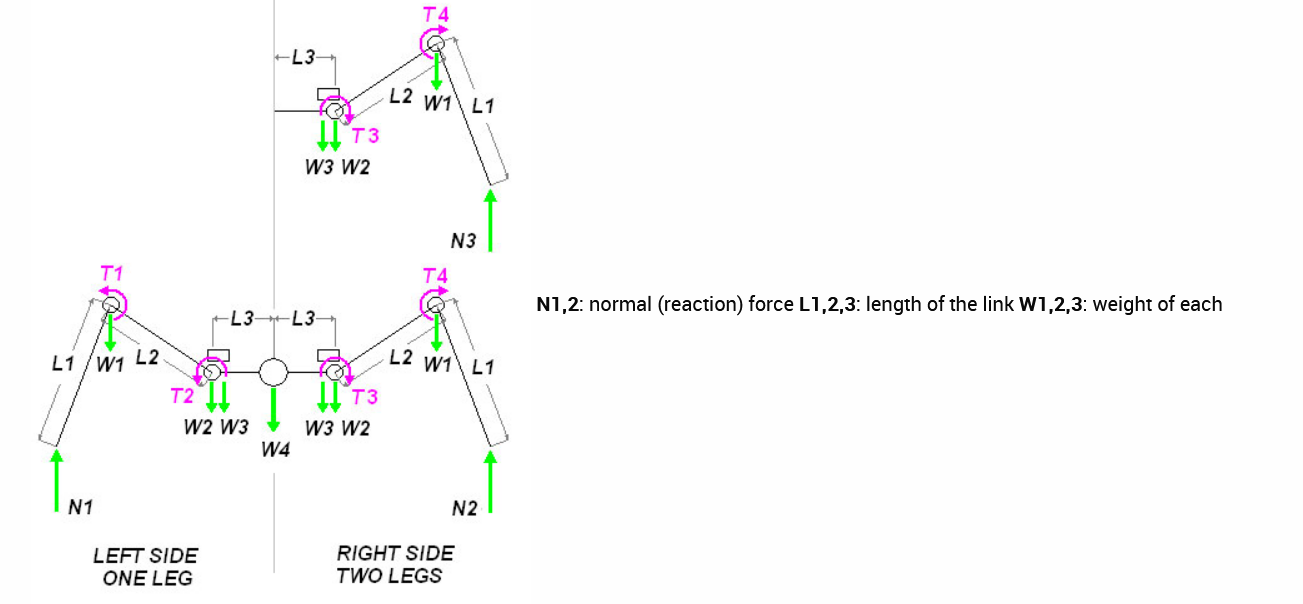
\includegraphics[width = 0.55\textwidth]{figures/1.png}                \caption{Hexapod diagram with assumptions made}
   \label{fig: Diagram 1}
\end{figure}

\begin{figure}
 \centering
   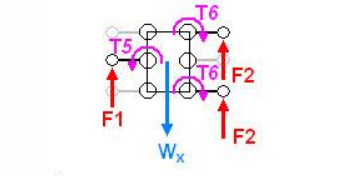
\includegraphics[width = 0.45\textwidth]{figures/2.png}
\caption{Diagram for horizontal motor torque of a hexapod.}
    \label{fig:Diagram 2}
\end{figure}

% The following declarations will create equations and automatically number them in the document. Notice the equation is given a unique name. You can reference these equations later in the document.


\subsection{Equations}
The was following assumption was made regarding the horizontal force on the hexapod using equation [\ref{eq: Horizontal Force Assumption}]
\begin{equation} \label{eq: Horizontal Force Assumption}
	F_1 = 2F_2
\end{equation}


The motor inertia was found using the formula  [\ref{eq: Motor Inertia}]
\begin{equation} \label{eq: Motor Inertia}
	J_{motor} = \frac{J_{load}}{n^2}
\end{equation}

	The first set of e quations focused on the motor inertia as well as the torque value of the model at critical positions along the frame. 
The horizontal motor was found using the formula below  [\ref{eq: Horizontal Motor Torque}]


\begin{multline} \label{eq: Horizontal Motor Torque}
\Sigma T_5 = T_1 - F_1 (L_1 \cos \theta_1 + L_2 \cos \theta_2) - L_3 W_x\\ + 2F_2 (2L_3 + L_1 \cos \theta_1 + L_2 \cos \theta_2)
\end{multline}

Another critical factor the torque on the upper leg was also calculated using the below listed formula [\ref{eq: Torque on Upper Arm}]

\begin{multline} \label{eq: Torque on Upper Arm}
	\Sigma T_{hip} = T_2 - N_1 (L_1 \cos \theta_1 + L_2 \cos \theta_2)\\ +
	W_1 (L_2 \cos \theta2) -W_4 L_3 -2W_2 L_3 - 2W_3 L_3\\ - 2W1 (2L_3 + L_2 \cos \theta_2)  + 	2N_2 (2L_3 + L_2 \cos \theta_2 + L_1 \cos \theta_1 )
\end{multline} 

The reaction force on one side of the hexapod for a single leg was represented as the torque for the foot of the leg and was calculated using the equation [\ref{eq: Torque on Foot}]

\begin{multline} \label{eq: Torque on Foot}
\Sigma T_{Left Foot} = -W_1 L_1 \cos \theta_1 - W_2 (L_1 \cos \theta_1 + L_2 \cos \theta_2)\\ - W_3 (L_1 \cos \theta_1 + L_2 \cos \theta_2) - W_4 ((L_1 \cos \theta_1 + L_2 \cos \theta_2 + L_3)\\ -2W_3 (2L_3 + L_1 \cos \theta_1 + L_2 \cos \theta_2)
- 2W_2 (L_1 \cos \theta_1 + L_2 \cos \theta_2 +2L_3)\\ - 2W_1 (L_1 \cos \theta_1 + 2L_2 \cos \theta_2 +2L_3)\\ + 2N_2 (2L_1 \cos \theta_1 + 2L_2 \cos \theta_2 +2L_3)
\end{multline}

The remaining reaction forces were calculated using the equation [\ref{eq: Reaction Forces}]
\begin{equation} \label{eq: Reaction Forces}
N_1+2N_2 = W_4+ 6(W_1+W_2+W_3 )
\end{equation}

The hexpods weight could be calculated as the summation of its component weights as can be seen in equation[\ref{eq: Weight}]

\begin{equation} \label{eq: Weight}
W_4 = W_{Frame}+W_{Battery}+W_{Elect}
\end{equation}


The hexapods incline control was determined using the following equation [\ref{eq: Incline Control}]

\begin{equation} \label{eq: Incline Control}
W_x = W \sin \beta
\end{equation}



\subsection{Solid works Model}
The results of these calculations along with the information from the design specifications were used to create the solid works model.

\begin{figure}[h]
 \centering
   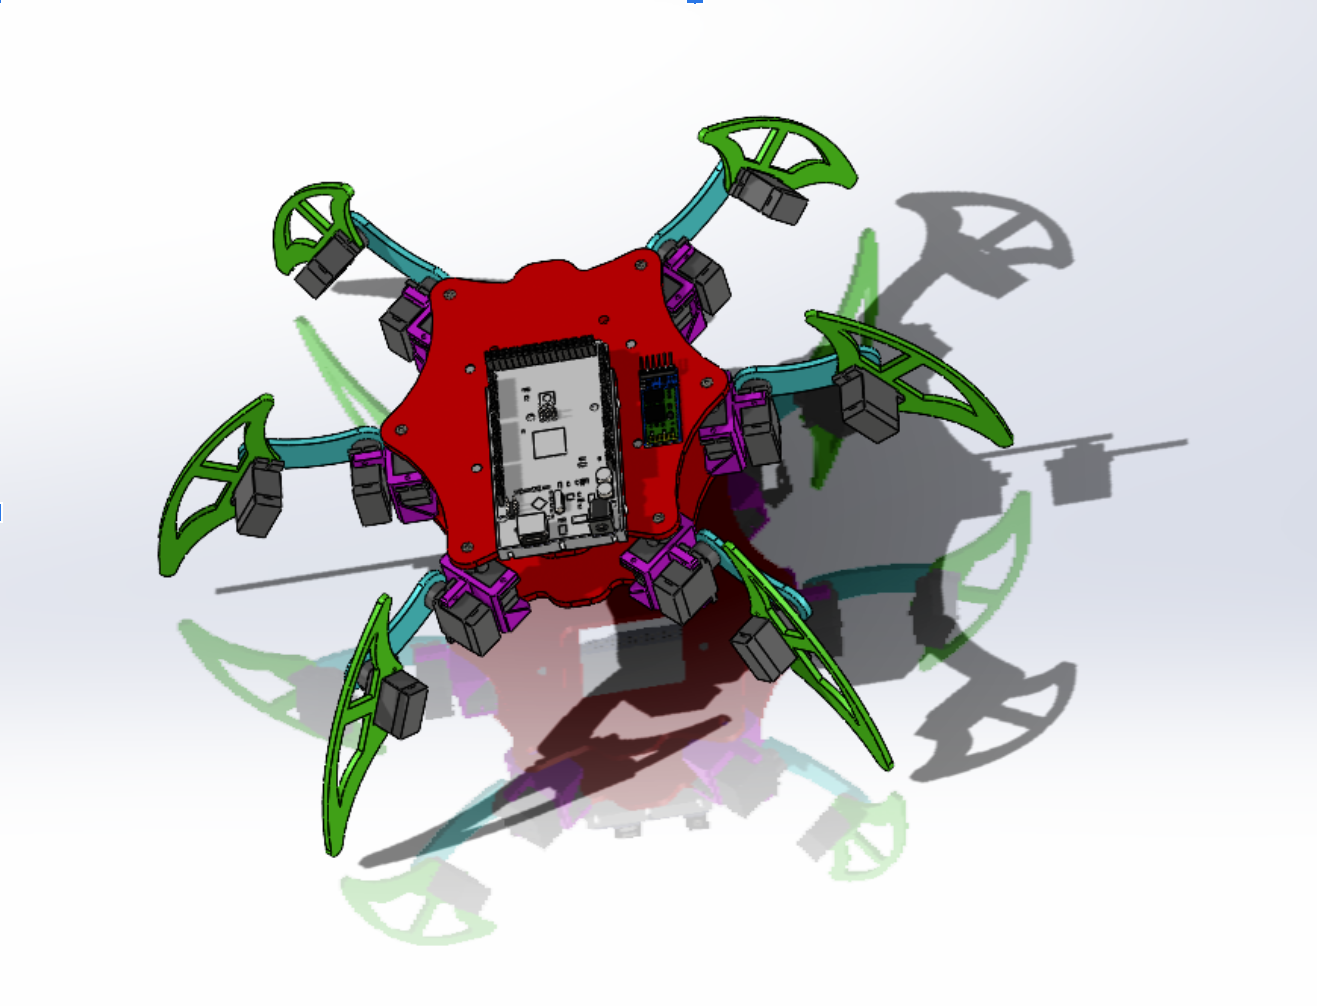
\includegraphics[width = 0.55\textwidth]{figures/3.png}                \caption{Hexapod Solidworks Model}
   \label{fig:Physical Model }
\end{figure}

The figure above depicts a hexapod developed with the core concepts above in mind. This hexapod robot is developed using PVC plastic. Using this mechanical model three core concepts were pulled for future use within the simulink model. The first is the structural safety factor determined from placing the mass of a third of the robot's weight (due to 3 legs up, 3 legs down) as a pressure upon a given test leg.The following table \ref{tab1} lists the design specifications of the solid works model

\begin{table}[htbp]
	\caption{Hexapod Dimensions}
	\begin{center}
		\begin{tabular}{|c|c|}
			\hline  
			Foot Mass & 20.18 g \\
			\hline
			Foot Length (L1) & 65.5 mm\\
			\hline
			Knee Mass (W1) & 57.54 g\\
			\hline
			Knee Length (L2) & 2 mm\\
			\hline
			Thigh Mass (W3) & 57.54 g\\
			\hline
			Arduino Mass (Warduino) & 47 g\\
			\hline
			Half Body Length (L3) & 79.72 mm\\
			\hline
			Full Body Mass (W4) & 598.06 g \\
		 	\hline
			
			
		\end{tabular}
		\end{center}
	\label{tab1}
	
\end{table}


Creating a model in solid works allowed us to perform simulations to determine values that would normally be difficult to calculate by hand for such an oddly shaped device. Using the solid works simulation we were able to observe the stress-strain relationship of our mechanical design.

\begin{figure}[h]
 \centering
   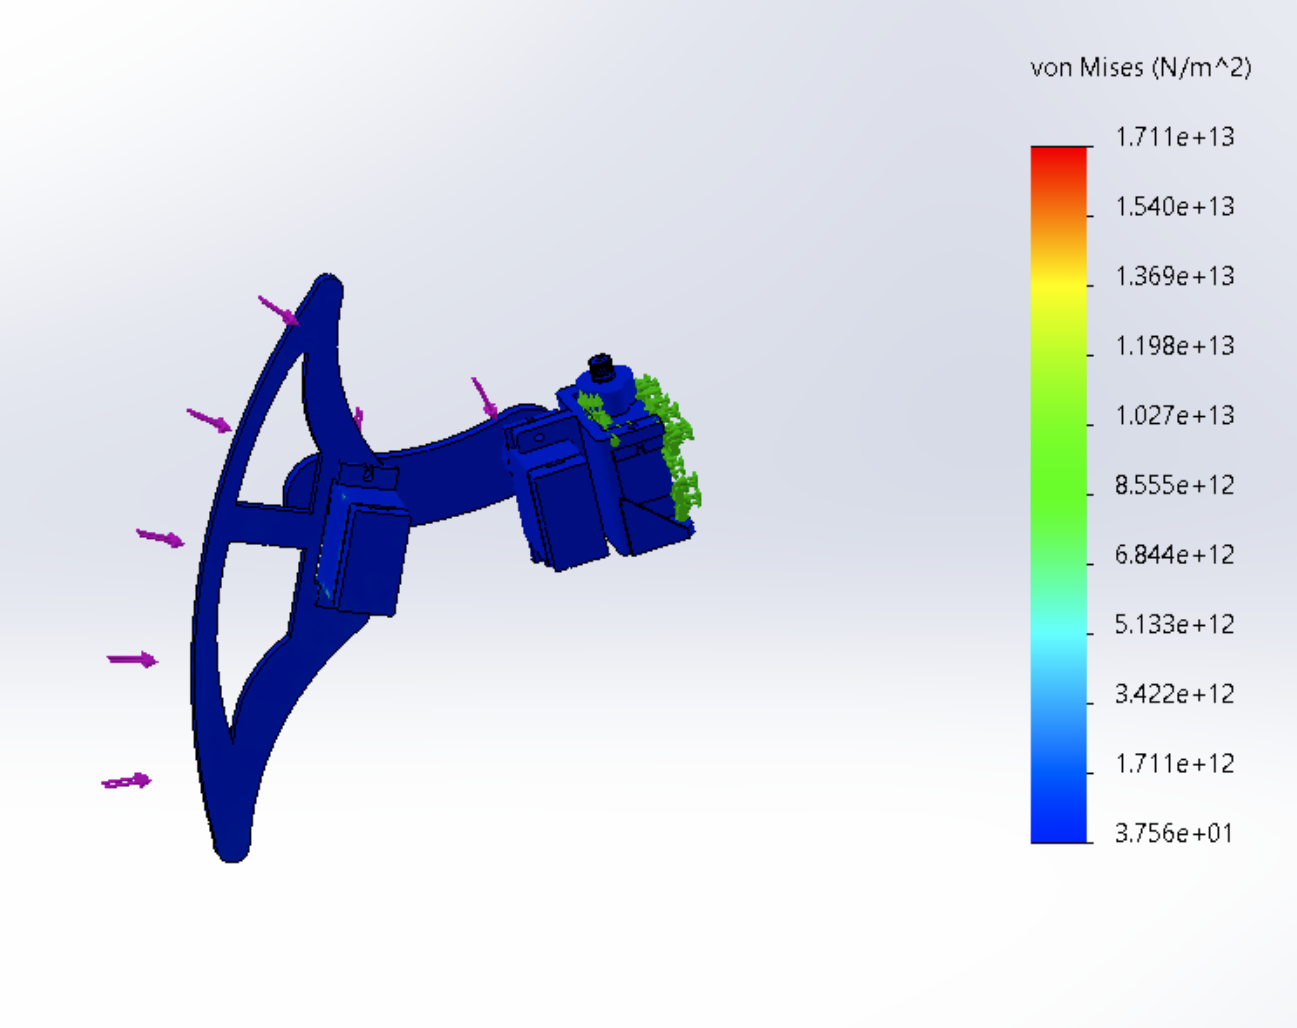
\includegraphics[width = 0.49\textwidth]{figures/4.png}                \caption{Stress-Strain of Mechanical Design}
   \label{fig:Stress-Strain of Mechanical Design}
\end{figure}



From the figure above it is determined that the model is structurally sound and thus is within the clear to perform test upon. Next we move onto understanding the specifications of each link and how they interact with each other. The solids works tool was used to determine the weights and lengths of each link; these values were later recorded for future use. As well the solids work model was then used to determine the range of motion the motors would be able to achieve. While the inertias could be hand solved using the formula in the matrix.\\

\begin{equation*}
I_c = 
\begin{bmatrix}
\frac{1}{12} M_c (3R^2+H^2) & 0 & 0\\
0 & \frac{1}{12} M_c R^2 & 0\\
0 & 0 & \frac{1}{12} M_c (3R^2+H^2)\\

\end{bmatrix}
\end{equation*}\\

It was determined that a solid works model could be used to simplify inertias within the 3 sets of components.\\

In order to understand the kinematic characteristics of a hexapod robot with arbitrary values imputed into link weights and link lengths we normally would use the Denavit-Hartenberg algorithm, applying it to a leg of the hexapod robot. Through the assumption that the model involved is a symmetrical structure composed of six identical legs, having three degrees of freedom in each leg we can thus assume due to symmetry that we only need to work on a single leg with a degree of freedom of 3 rather then the complete model with a degree of freedom of 18.

% For an equation in line with text use the following. Note that these types of equations will not be numbered. Also note the use of "$" sign.
%You can reference the equations above in your document by using their defined label, [\ref{eq: TransientCurrent}] and [\ref{eq: SteadyStateCurrent}]. Steady-state: $I_0= i_0(\omega t =0) = i_0(\omega t = \pi)$. Individual variables can also be called, such as $\omega_0$. 

\subsection{Electromechanical Model in Simulink}
Once the necessaey calculations an physical modelling had been complete the project continued with the design of the Electromechanical model using simulink simulation software.\\

Before the models construction,research had first been conducted on various servo motors and their performance as well as subsequent electro mechanical models. Figures \ref{fig:Model of DC motor with external load coupled by gears} and \ref{fig:Model Showing Load Effect on motor} represent the load effects on the system .\\

\begin{figure}[h]
 \centering
   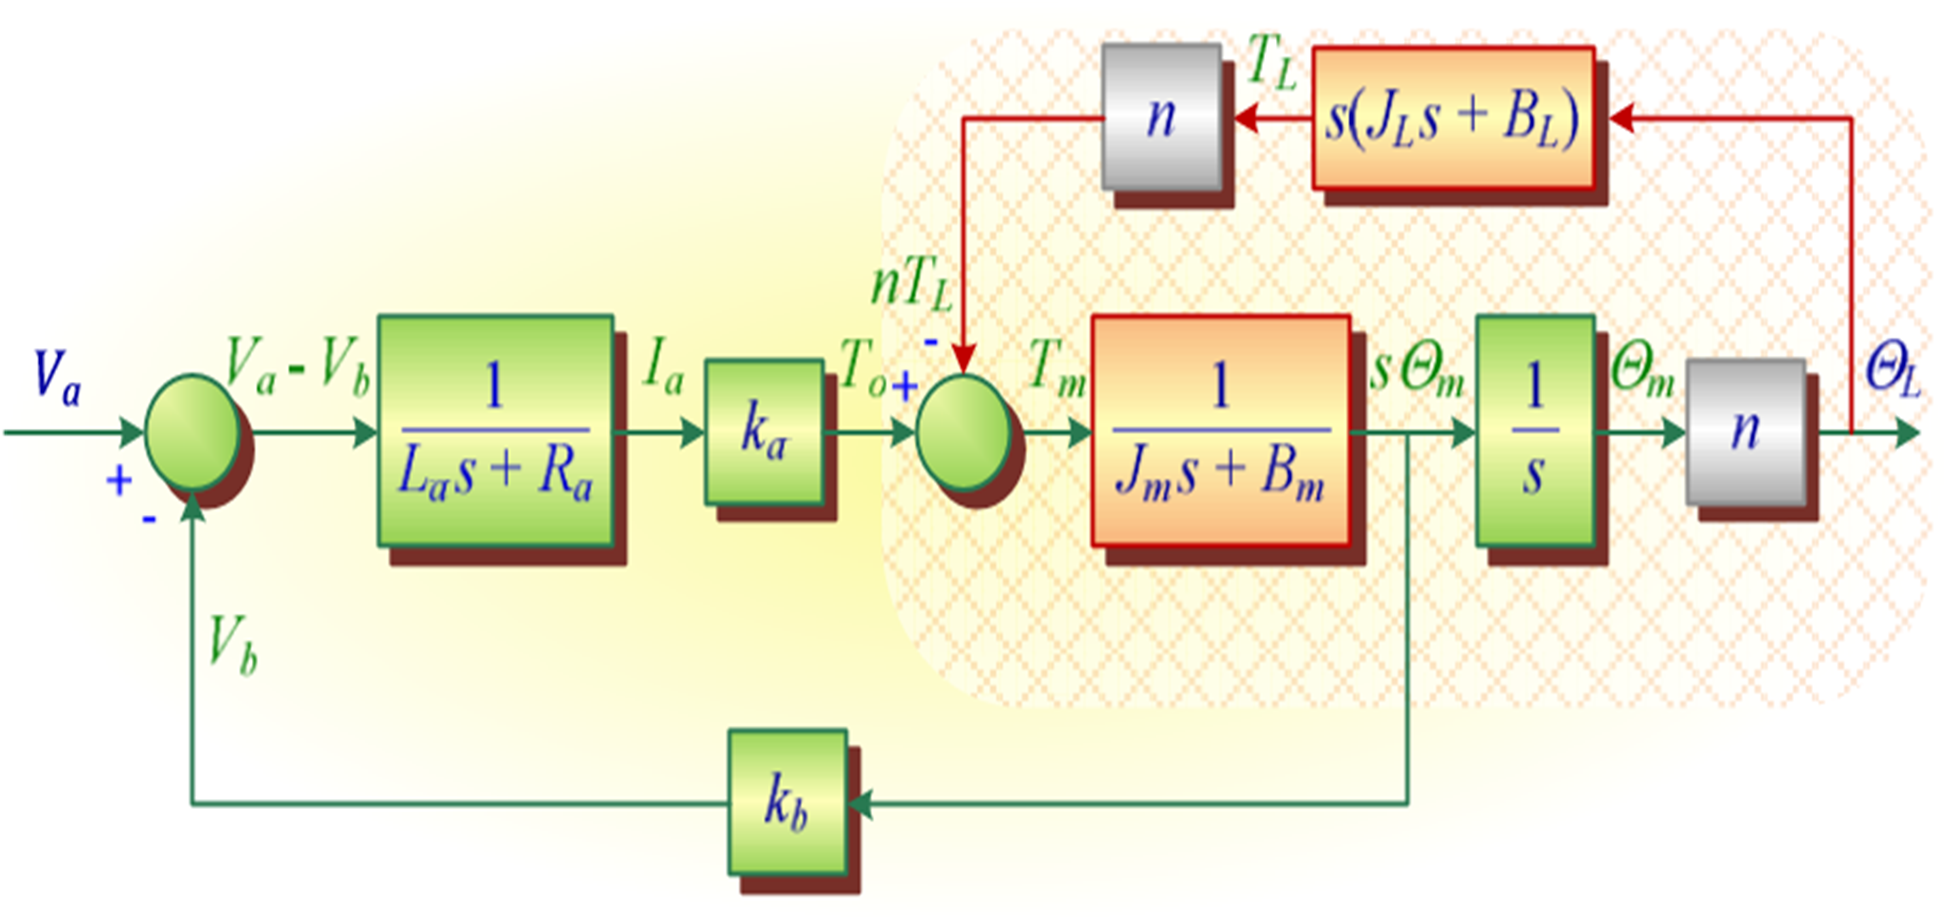
\includegraphics[width = 0.5\textwidth]{figures/5.png}                \caption{Model of DC motor with external load coupled by gears}
   \label{fig:Model of DC motor with external load coupled by gears}
\end{figure}

\begin{figure}[h]
 \centering
   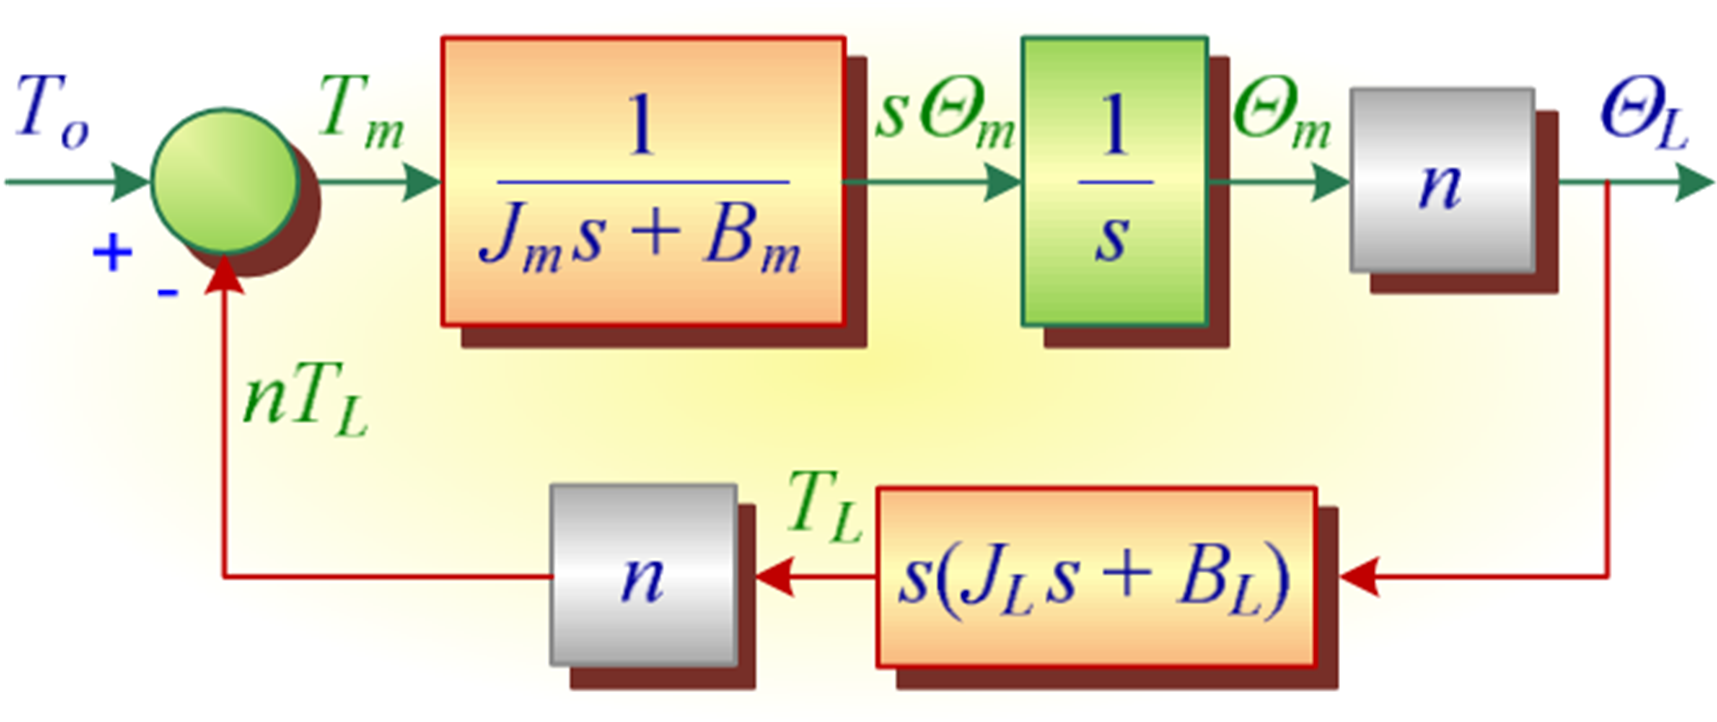
\includegraphics[width = 0.5\textwidth]{figures/6.png}                \caption{Model showing load effect on motor}
   \label{fig:Model Showing Load Effect on motor}
\end{figure}





Once the necessary research had been conducted the electromechanical model was designed as can be seen in figure \ref{fig:Electromechanical Model}


\begin{figure}[H]
 \centering
   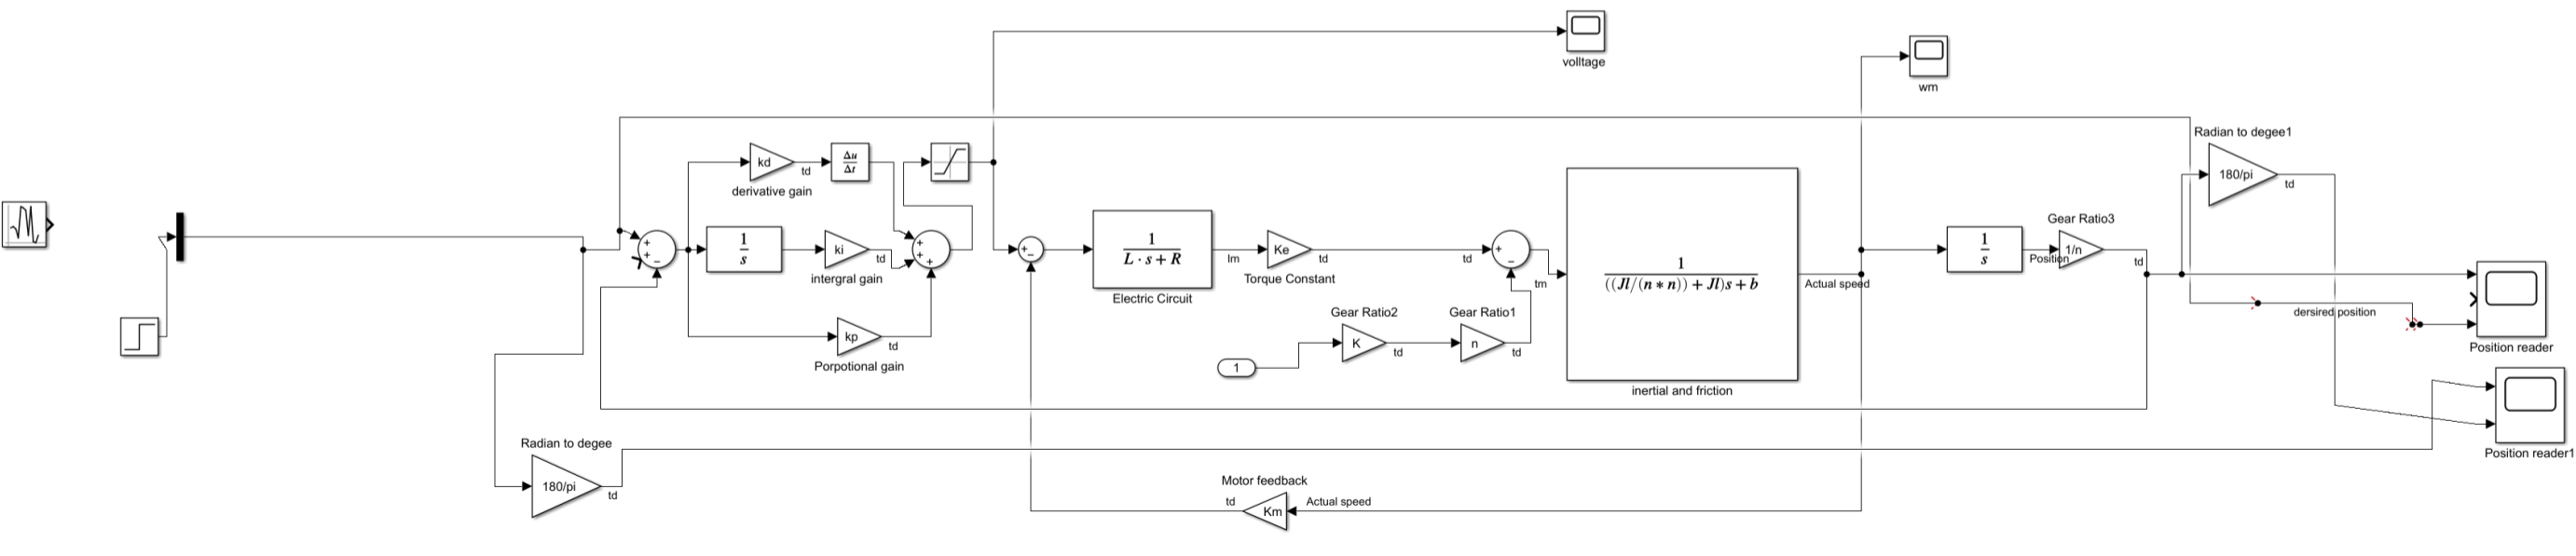
\includegraphics[width = 0.45\textwidth]{figures/7.png}  \caption{Electromechanical Model of servo motor}
   \label{fig:Electromechanical Model}
\end{figure}
The model of the servo motor in figure \ref{fig:Electromechanical Model} uses a PID controller to measure the difference in desired and current position adjusting the voltage output accordingly. It should be noted that the servo motor would also include a potentiometer represented by a block relating voltage to angular position and a pulse with signal, however is was assumed that the pulse with would be generated by the micro controller and their by making creation of the pulse with and by extension the potentiometer relating to it not necessary.
During testing the PID controller and gearbox were the only variable tuned as all other variables had been calculated from data sheet and experimental with reference 9g servo model. Both the Kp and gear box were increment together as the kp decreased response time contracting the gearboxes effect on load torque, a Kd value was included to minimize overshoot. Due to the high kp value it was decided to add a saturation block to represent the motoring reaching its max input voltage saturation to allow the model to remain plausible. Though simulation results shown in figure \ref{fig:Electromechanical Model Simulation Results} and figure \ref{fig:Electromechanical Model Simulation varying input positions} Model Simulation varying input positions} it was concluded that the created motor was able to proved a response time of 0.177 seconds for a 60 degree change and over multiple changes in position was able to average a overshoot of 3 percent each time. 
\begin{figure}[h]
 \centering
   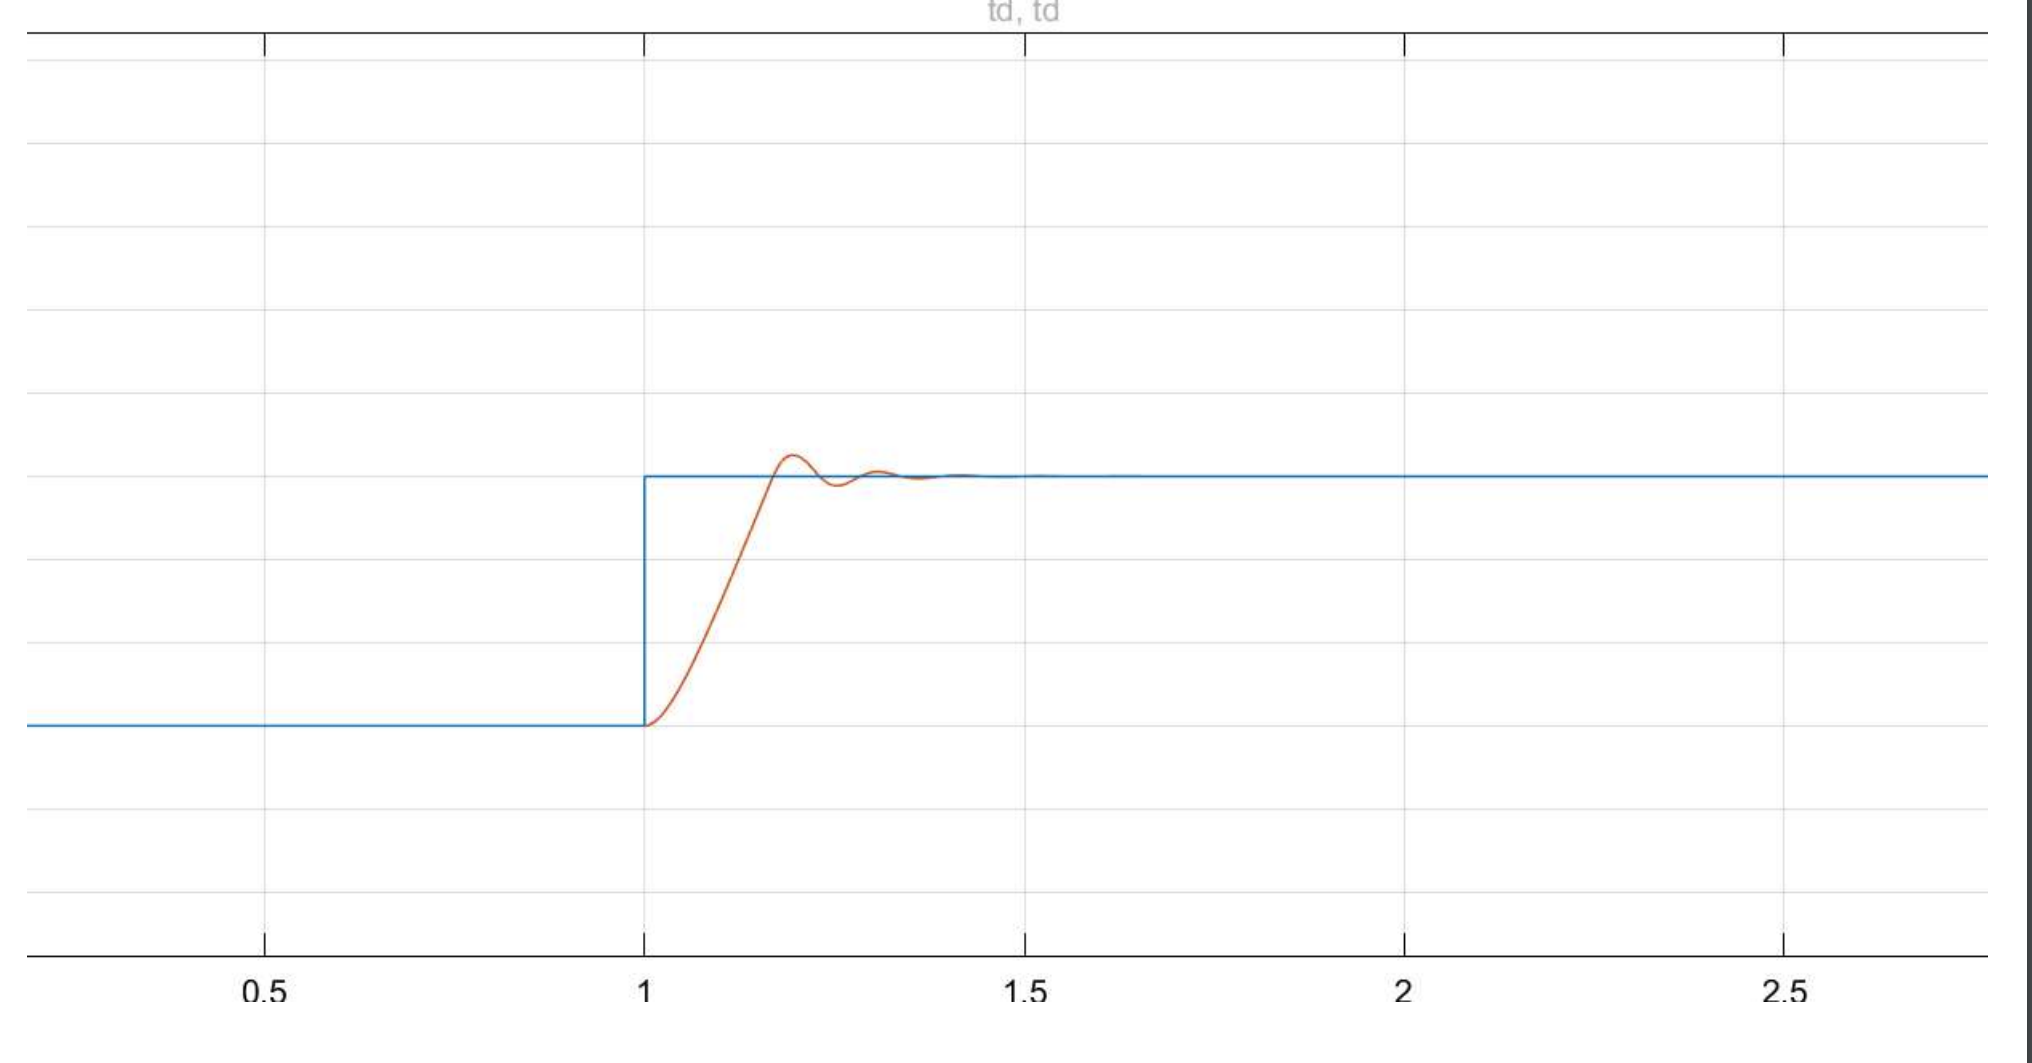
\includegraphics[width = 0.45\textwidth]{figures/8.png}                \caption{Electromechanical Model Simulation Results}
   \label{fig:Electromechanical Model Simulation Results}
\end{figure}
\begin{figure}[h]
 \centering
   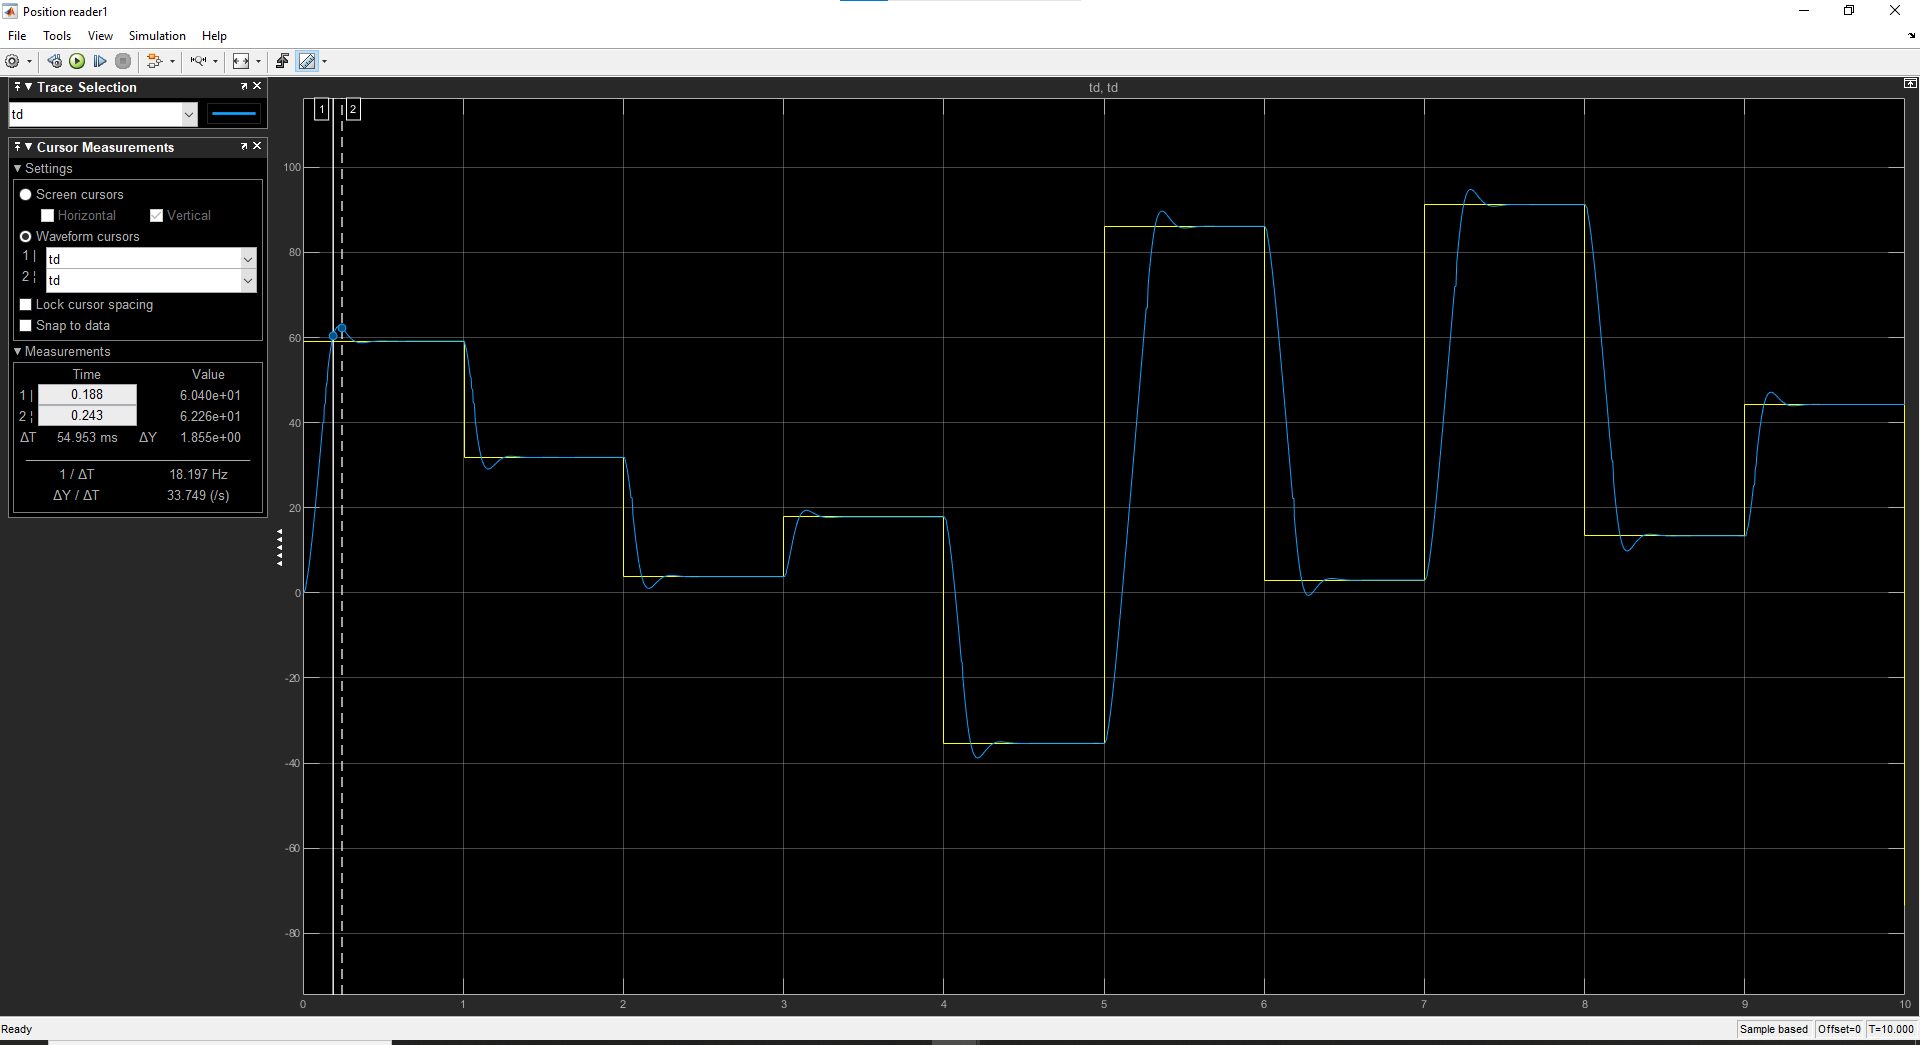
\includegraphics[width = 0.45\textwidth]{figures/9.png}                \caption{Electromechanical Model Simulation Results}
   \label{fig:Electromechanical Model Simulation varying input positions}
\end{figure}







%Figure Labels: Use words rather than symbols or abbreviations when writing Figure axis labels to avoid confusing the reader. As an example, write the quantity ``Magnetization'', or ``Magnetization, M'', not just ``M''. If including units in the label, present them within parentheses. Do not label axes only with units. In the example, write ``Magnetization (A/m)'' or ``Magnetization \{A[m(1)]\}'', not just ``A/m''. Do not label axes with a ratio of quantities and units. For example, write ``Temperature (K)'', not ``Temperature/K''. See examples Fig. \ref{fig:mySampleFigure} and Fig. \ref{fig:myOtherSampleFigure} in this document.

%All figures should be clearly explained in the text. Furthermore, all figures should have a purpose, do not include irrelevant or redundant images. Doing so will only make the document more cluttered.














%% --------------------------------   Sub: References  --------------------------------
% You do not need to individually number your citations, for example typing [1]. Make use of the \cite command. 
% Your citations will be automatically numbered when using \cite. This also makes constructing your bibliography later easier.
% It is strongly encouraged to use Google Scholar and Bibtex to create your .bib file.
\subsection{References}
The value outlines how to properly include citations in your report. The sources used are only used in an example context.
Please number citations consecutively within brackets \cite{halter2008electrical}. The sentence punctuation follows the bracket \cite{jossinet1998impedivity}. Refer simply to the reference number, as in \cite{cole1941dispersion}---do not use ``Ref. \cite{cole1941dispersion}'' or ``reference \cite{cole1941dispersion}'' except at the beginning of a sentence: ``Reference \cite{cole1941dispersion} was the first $\ldots$''



Number footnotes separately in superscripts. Place the actual footnote at 
the bottom of the column in which it was cited. Do not put footnotes in the 
abstract or reference list. Use letters for table footnotes.



Unless there are six authors or more give all authors' names; do not use 
``et al.''. Papers that have not been published, even if they have been 
submitted for publication, should be cited as ``unpublished'' \cite{gabriel1996dielectricI}. Papers 
that have been accepted for publication should be cited as ``in press'' \cite{gabriel1996dielectricI}. 
Capitalize only the first word in a paper title, except for proper nouns and 
element symbols.



For papers published in translation journals, please give the English 
citation first, followed by the original foreign-language citation \cite{khadem2019geometric}.












%% --------------------------------   Conclusion  --------------------------------
\section{Conclusion and Discussion}
%/The conclusion should be used to address the success of your design. Answer and discuss if your design met the requirements, had good performance, etc. If applicable, suggest future improvements or applications of the design.


Upon the completion of this project an understanding of electromcechanical system control specifically with hexapods was developed. This 



% Construct references section.
\bibliographystyle{IEEEtran}
\bibliography{myWorksCited}




\end{document}
